\nonstopmode

\documentclass[letterpaper,12pt,titlepage]{report}
\usepackage{amsthm,amssymb}
\usepackage{mathtools}
\mathtoolsset{showonlyrefs}
\usepackage{bm}
\usepackage[margin=1in]{geometry}
\usepackage{booktabs}
\usepackage{enumitem}
\usepackage{framed}
\usepackage{tikz}
\usetikzlibrary{shapes,arrows.meta,positioning,patterns,calc,decorations.pathmorphing}
\usepackage{pgfplots}
\pgfplotsset{compat=1.9}
\usepackage{algpseudocode}
\usepackage{algorithm}

\usepackage[pdfpagelabels]{hyperref}

\usepackage{fancyhdr}
\pagestyle{fancy}
\fancyhead{}
\fancyfoot{}
\fancyfoot[L]{K.\ Okkelberg}
\fancyfoot[R]{\thepage}
\renewcommand{\headrulewidth}{0pt}
\renewcommand{\footrulewidth}{0.5pt}

\newcommand*\dif{\mathop{}\!\mathrm{d}}
\newcommand{\trans}{^\text{T}}
\newcommand{\herm}{^\text{H}}
\DeclareMathOperator{\E}{E}
\DeclareMathOperator{\trace}{trace}
\DeclareMathOperator{\sign}{sign}
\let\Pr\relax
\DeclareMathOperator{\Pr}{P}
\newcommand*\pder[2]{\frac{\partial #1}{\partial #2}}
\newcommand*\R{\mathbb{R}}
\newcommand*\U{\mathcal{U}}

\theoremstyle{plain}
\newtheorem*{thm}{Theorem}
\theoremstyle{definition}
\newtheorem*{defi}{Definition}

\tikzstyle{line} = [draw, thick, >=latex]
\tikzstyle{dot} = [circle,fill=black,inner sep=0pt,minimum size=4pt]
\tikzset{>=latex}

\begin{document}

\hypersetup{pageanchor=false}
\title{ECE 6553: Optimal Control Notes}
\author{Klaus Z.\ Okkelberg}
\date{Spring 2017}
\maketitle
\hypersetup{pageanchor=true}

\chapter{Parameter Optimization}

% 2017/01/10
\section{What is optimal control?}
\paragraph{Optimal} Maximize/minimize cost (subject to constraints): $ \min_u g(u) $

With constraints,
\begin{align}
  \min_u {}\ & g(u) \\
  \text{s.t. } & \begin{cases} h_1(u) = 0 \\ h_2(u) \le 0 \end{cases}
\end{align}

First-order necessary condition (FONC):
\[ \frac{\partial g}{\partial u}(u^*) = 0 \]

Optimality can be
\begin{itemize}
\item local vs global
\item max vs min
\end{itemize}

\begin{center}
  \begin{tikzpicture}
    \draw [thick,->] (0,0) -- (0,4) node [anchor=east] {$g$};
    \draw [thick,->] (0,0) -- (6.5,0) node [anchor=north west] {$u$};
    \draw plot [smooth, tension=1] coordinates { (0.5,3) (2,0.5) (3.5,3) (4.25,1) (5,2) (5.5,1.5) (6,2) };
    \draw [thick] (2,0.1) -- (2,-0.1) node [anchor=north] {$u^*$};
  \end{tikzpicture}
\end{center}

\paragraph{Control} control design: pick $u$ such that specifications are satisfied:
\[ \dot{x} = f(x,u), \qquad \dot{x} = Ax + Bu, \]
where $x(t)\in\mathbb{R}^n$ is the state, $u(t)\in\mathbb{R}^m$ is the control, and $f(\cdot)$ is the dynamics.

Actually, $x$ and $u$ are signals:
\[ x:[0,T]\to\R^n, \qquad  u:[0,T]\to\R^m \]

\paragraph{Optimal control} find the ``best'' u!

For ``best'' to mean anything, we need a cost. The big/deep question is
\[ \frac{\partial \text{``cost''}}{\partial u} = 0 \]

\paragraph{Example} \mbox{}

Suppose we have a car with position $p$. Its acceleration $\ddot{p}$ is controlled by the gas/brake input $u$ ($\ddot{p}=u$). In order to express the dynamics of the system in the form $\dot{x}=f(x,u)$, we introduce state variables:
\[
  \begin{aligned} x_1 &= p \\ x_2 &= \dot{p} \end{aligned}
  \ \Longrightarrow \
  \begin{cases} \dot{x}_1 = x_2 \\ \dot{x}_2 = u \end{cases}
\]
The task is to move the car from its initial position to a stop at a distance $c$ away.

\subparagraph{Minimum energy problem}
\begin{align}
  \min_u {}\ & \int_0^T\! u^2(t) \dif t \\
  \text{s.t. } & \begin{cases} \dot{x}_1 = x_2 \\ \dot{x}_2 = u \end{cases} \\
             & x_1(0) = 0,\, x_2(0) = 0 \\
             & x_1(T) = c,\, x_2(T) = 0
\end{align}

\subparagraph{Minimum time problem}
\begin{align}
  \min_{u,T} {}\ & T = \int_0^T\! \dif t \\
  \text{s.t. } & \begin{cases} \dot{x}_1 = x_2 \\ \dot{x}_2 = u \end{cases} \\
                 & x_1(0) = 0,\, x_2(0) = 0 \\
                 & x_1(T) = c,\, x_2(T) = 0 \\
                 & u(t) \in [u_\text{min},u_\text{max}]
\end{align}

The general optimal control problem we will solve will look like
\begin{align}
  \min_{u,T} {}\ & \int_0^T\! L(x(t),u(t),t) \dif t + \Psi(x(T)) \\
  \text{s.t. } & \dot{x}(t) = f(x(t),u(t),t),\ t\in[0,T] \\
                 & x(0) = x_0 \\
                 & x(T) \in S \\
                 & u(t) \in \Omega,\ t\in[0,T]
\end{align}
where $\Psi(\cdot)$ is the terminal cost and $S$ is the terminal manifold. This is a so-called \textbf{Bolza Problem}.

\paragraph{What tools do we need to solve this?}
\begin{enumerate}
\item optimality conditions $\partial\text{cost}/\partial u=0$
\item some way of representing the optimal signal $u^*(x,t)$
\item some way of actually finding/computing the optimal controllers
\end{enumerate}

% 2017/01/12
\section{Unconstrained Optimization}

Let the decision variable be $u=[u_1, \dots, u_m]\trans\in\mathbb R^m$. The cost is $g(u)\in C^1$ ($C^k$ means $k$ times continuously differentiable). The problem is
\[ \min_u g(u), \quad g:\mathbb R^m \to \mathbb R \]
For $u^*$ to be a minimizer, we need
\[ \pder{g}{u} (u^*) = 0 \]
\begin{defi}
  $u^*$ is a (local) minimizer to $g$ if $\exists\delta>0$ s.t.
  \begin{gather}
    g(u^*) \le g(u) \quad \forall u\in B_\delta(u^*) \\
    B_\delta(u^*) = \{ u \mid \Vert u-u^* \Vert \le \delta \}
  \end{gather}
\end{defi}

\paragraph{Note:} \mbox{}
\begin{itemize}
\item $\displaystyle \pder{g}{u}(u^*) \delta u \in \mathbb R$ and $\delta u$ is $m\times 1$, so $\displaystyle \pder{g}{u}$ is a $1\times m$ row vector. For the column vector,
  \[ \nabla g = \pder{g\trans}{u} \in \mathbb R^m \]
\item $\displaystyle \pder{g}{u} \, \delta u$ is an inner product
  \[ \langle \nabla g, \delta u \rangle = \left\langle \pder{g\trans}{u}, \delta u \right\rangle \]
\item $o(\varepsilon)$ encodes higher-order terms
  \[ \lim_{\varepsilon\to 0} \frac{o(\varepsilon)}{\varepsilon} = 0 \qquad \text{``faster than linear''} \]
  This is opposed to big-O notation:
  \[ \lim_{\varepsilon\to 0} \frac{\mathcal O(\varepsilon)}{\varepsilon} = c \]
\item $\delta u$ has direction and scale so we could write it as
  \[ \delta u = \varepsilon v, \quad \varepsilon\in\mathbb R,\ v\in\mathbb R^m \]
\end{itemize}

\begin{thm}
  For $u^*$ to be a minimizer, we need
  \[ \pder{g}{u} (u^*) = 0 \]
  or, equivalently,
  \[ \pder{g}{u} (u^*) v = 0 \quad \forall v\in\mathbb R^m \]
\end{thm}

\begin{proof}
  Let $u^*$ be a minimizer. Evaluating the cost $g(u)$ in the ball and using Taylor's expansion,
  \[ g(u^* + \delta u) = g(u^*) + \pder{g}{u} (u^*) \delta u + o(\Vert\delta u\Vert) = g(u^*) + \varepsilon \pder{g}{u} (u^*) v + o(\varepsilon) \]
  Assume that $\pder{g}{u} \neq 0$. Then we could pick $v=-\pder{g\trans}{u}(u^*)$, i.e.
  \[ g(u^*+\varepsilon v) = g(u^*) - \varepsilon \left\Vert \pder{g\trans}{u} (u^*) \right\Vert^2 + o(\varepsilon) \]
  Note that the second term is negative per our assumptions. So, for $\varepsilon$ sufficiently small, we have
  \[ g \Big( u^* - \varepsilon\pder{g\trans}{u} (u^*) \Big) < g(u^*) \]
  This contradicts $u^*$ being a minimizer. \quad
  
\begin{tikzpicture}[scale=0.3]
    \draw (0,0) -- (1,1);
    \draw (0,1) -- (1,0);
    \draw (0,0.35) -- (0.35,0);
    \draw (0.65,0) -- (1,0.35);
  \end{tikzpicture}
  (crossed swords)
\end{proof}

\begin{defi}[Positive definite]
  $M=M\trans \succ 0$ if
  \begin{gather}
    z\trans M z > 0 \quad \forall z\neq 0,\ z\in\mathbb R^m \\
    \Longleftrightarrow M \text{ has real and positive eigenvalues}
  \end{gather}
\end{defi}

\begin{thm}
  If $g\in C^2$, then a \textbf{sufficient} condition for $u^*$ to be a (local) minimizer is
  \begin{enumerate}
  \item $\displaystyle \pder{g}{u}(u^*) = 0$
  \item $\displaystyle \pder{^2 g}{u^2}(u^*) \succ 0$ (the Hessian is positive definite)
  \end{enumerate}
\end{thm}

\begin{defi}
  $g:\mathbb R^m\to\mathbb R$ is convex if
  \[ g(\alpha u_1 + (1-\alpha)u_2) \le \alpha g(u_1) + (1-\alpha)g(u_2) \quad \forall \alpha\in[0,1], \ u_1,\! u_2\in\mathbb R^m \]
  \begin{center}
    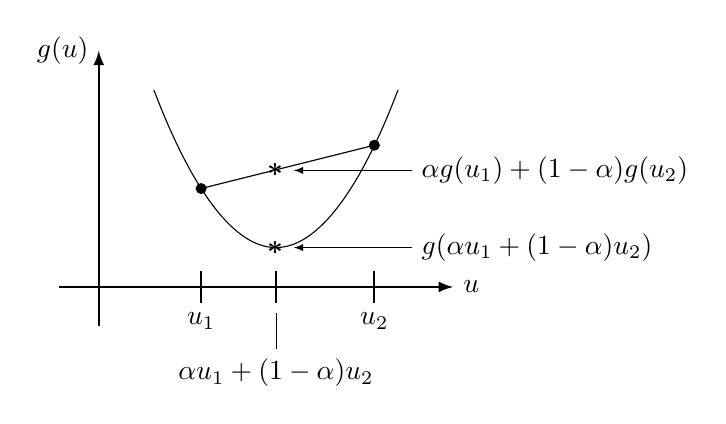
\begin{tikzpicture}
      \path [line,->] (-0.5,0) -- (4.5,0) node [anchor=west] {$u$};
      \path [line,->] (0,-0.5) -- (0,3) node [anchor=east] {$g(u)$};
      \draw (0.7,2.5) parabola bend (2.25,0.5) (3.8,2.5);
      \path [line] (1.3,-0.2) node [anchor=north] {$u_1$} -- (1.3,0.2);
      \path [line] (3.5,-0.2) node [anchor=north] {$u_2$} -- (3.5,0.2);
      \path [line] (2.25,-0.2) node [pin={[pin edge={black}] below:{$\alpha u_1 + (1-\alpha)u_2$}}] {} -- (2.25,0.2);
      \draw (1.3,1.25) -- (3.5,1.8);
      \fill (1.3,1.25) circle (0.07);
      \fill (3.5,1.8) circle (0.07);
      \node [pin={[pin edge={black,<-},pin distance=1.5cm] right:{$g(\alpha u_1 + (1-\alpha)u_2)$}}] at (2.25,0.5) {$\bm *$};
      \node [pin={[pin edge={black,<-},pin distance=1.5cm] right:{$\alpha g(u_1) + (1-\alpha)g(u_2)$}}] at (2.25,1.48) {$\bm *$};
    \end{tikzpicture}
  \end{center}
\end{defi}

\begin{thm}
  If $\pder{^2 g}{u^2} (u) \succeq 0$ $\forall u\in\mathbb R^m$, then $g$ is convex. ($\Longleftrightarrow$ for $g\in C^2$)
\end{thm}

\paragraph{Example} $\displaystyle \min_u u\trans Q u - b\trans u$ where $Q=Q\trans\succ 0$ (positive definite matrix)
\begin{align}
  \pder{g}{u} &= \pder{}{u} (u\trans Qu - b\trans u) \\
              &= u\trans Q\trans + u\trans Q - b\trans \\
              &= 2u\trans Q - b\trans \\[-3ex]
  \pder{^2 g}{u^2} &= 2Q
              & \pder{^2 g}{u^2} = \begin{bmatrix}
                \pder{^2 g}{u_1^2} & \cdots & \pder{^2 g}{u_1 \partial u_m} \\
                \vdots & \ddots & \vdots \\
                \pder{^2 g}{u_m \partial u_1} & \cdots & \pder{^2 g}{u_m^2}
              \end{bmatrix}
\end{align}
From $\pder{g}{u} = 2u\trans Q-b\trans = 0$,
\[ u = \frac12 Q^{-1} b \]
To see whether this is a minimizer, consider the Hessian. Since $Q \succ 0$, it follows that $\pder{^2 g}{u^2} (u^*) \succ 0$ and $u^*=\frac12 Q^{-1} b$ is a (local) minimizer. Additionally, since $\pder{^2 g}{u^2} \succ 0$, $g$ is convex and $u^*$ is a global minimizer. In fact, since we have strict convexity ($\succ 0$ rather than $\succeq 0$), it is the unique global minimizer.

In optimal control, \emph{local} is typically all we can ask for. In optimization, we can do better!

But wait, just because we know $\pder{g}{u}=0$, it doesn't follow that we can actually find $u^*$\dots

\section{Numerical Methods}
Idea: $u_{k+1}=u_k+\text{step}_k$. What should $\text{step}_k$ be? For small $\text{step}_k=\gamma_k v_k$,
\[ g(u_k \cdot \text{step}_k) = g(u_k) + \pder{g}{u}(u_k) \cdot \text{step}_k + o(\Vert \text{step}_k \Vert) = g(u_k) + \gamma_k \pder{g}{u}(u_k) v_k + o(\gamma_k) \]
A perfectly reasonable choice of step direction is
\[ v_k=-\pder{g\trans}{u}(u_k), \]
known as the \emph{steepest descend} direction. This produces
\[ g \Big( u_k - \gamma_k\pder{g}{u}(u_k) \Big) = g(u_k) - \gamma_k \left\Vert \pder{g}{u}(u_k) \right\Vert^2 + o(\gamma_k) \]

\begin{framed}
  \textbf{Steepest descent} \[ u_{k+1} = u_k - \gamma_k \pder{g\trans}{u} (u_k) \]
\end{framed}

\paragraph{Note:} \mbox{}
\begin{itemize}
\item What should $\gamma_k$ be?
\item This method ``pretends'' that $g(u)$ is linear. If we pretend $g(u)$ is quadratic, we get
  \[ u_{k+1} = u_k - \left( \pder{^2 g}{u^2} (u_k) \right)^{-1} \pder{g\trans}{u} (u_k), \]
  i.e.\ Newton's Method
\end{itemize}

\paragraph{This course:} steepest descent

\subparagraph{Step-size selection?} \mbox{}
\begin{itemize}
\item Choice 1: $\gamma_k=\gamma$ ``small'' $\forall k$; will get close to a minimizer if $u_0$ is close enough and $\gamma$ small enough

  Problems: \vspace{-1ex}
  \begin{itemize}
  \item You may not converge! (but you'll get close)
  \item You may go off to infinity (diverge)
  \end{itemize}

  \begin{center}
    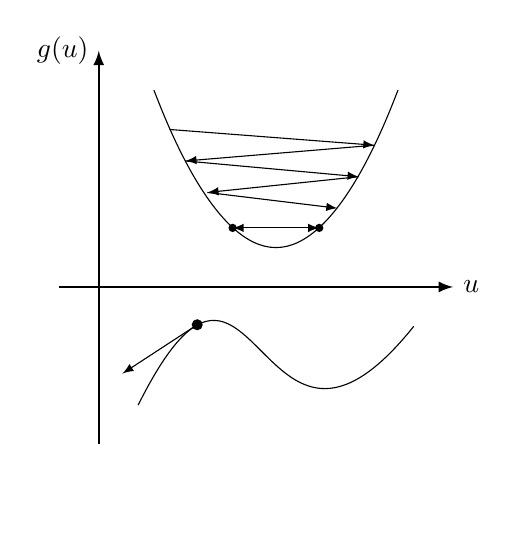
\begin{tikzpicture}
      \path [line,->] (-0.5,0) -- (4.5,0) node [anchor=west] {$u$};
      \path [line,->] (0,-2) -- (0,3) node [anchor=east] {$g(u)$};
      \draw (0.7,2.5) parabola bend (2.25,0.5) (3.8,2.5);
      \draw (0.5,-1.5) .. controls (2,1.5) and (2,-3) .. (4,-0.5);

      \draw [<->,>=latex] (1.7,0.75) node [circle,fill=black,minimum size=3pt,inner sep=0pt] {} -- (2.8,0.75) node [circle,fill=black,minimum size=3pt,inner sep=0pt] {};

      \draw [->,>=latex] (0.9,2) -- (3.5,1.8);
      \draw [->,>=latex] (3.5,1.8) -- (1.1,1.6);
      \draw [->,>=latex] (1.1,1.6) -- (3.3,1.4);
      \draw [->,>=latex] (3.3,1.4) -- (1.38,1.2);
      \draw [->,>=latex] (1.38,1.2) -- (3.03,1);

      \draw [->,>=latex] (1.25,-0.48) node [circle,fill=black,inner sep=0pt,minimum size=4pt] {} -- (0.3,-1.1);
    \end{tikzpicture}
  \end{center}
  
\item Choice 2: Reduce $\gamma_k$ as a function of $k$; will get close to a minimizer if $u_0$ is close enough

  Problem: slow

  \begin{thm}
    If $u_0$ is close enough to $u^*$ and $\gamma_k$ satisfies
    \begin{itemize}
    \item $\displaystyle \sum_{k=0}^\infty \gamma_k = \infty$
    \item $\displaystyle \sum_{k=0}^\infty \gamma_k^2 < \infty$
    \end{itemize}
    e.g.\ $\gamma_k=c/k$, then $u_k\to u^*$ as $k\to\infty$.
  \end{thm}
  
  % 2017/01/17
\item Choice 3: \textbf{Armijo step-size:} Take as big a step as possible, but no larger

  Pick $\alpha\in(0,1)$, $\beta\in(0,1)$. Let $i$ be the smallest non-negative integer such that
  \begin{gather}
    g\left( u_k - \beta^i \pder{g\trans}{u}(u_k) \right) - g(u_k) < -\alpha\beta^i \left\Vert \pder{g}{u}(u_k) \right\Vert^2 \\
    u_{k+1} = u_k - \beta^i \pder{g\trans}{u}(u_k)
  \end{gather}
  This will get to a minimizer blazingly fast if $u_0$ is close enough.
\end{itemize}

\section{Constrained Optimization}

Equality constraints:
\begin{align}
  \min_{u\in\mathcal R^m} {}\ & g(u) \\
  \text{s.t. } & h(u)=\bm 0
\end{align}
Consider $u\in\mathbb R^2$, $h:\mathbb R^2\to\mathbb R$
\begin{center}
  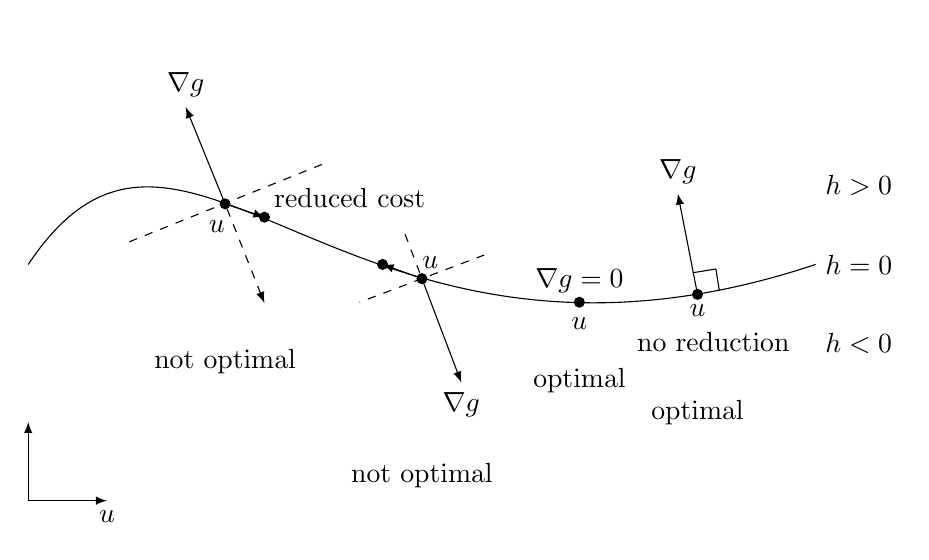
\begin{tikzpicture}[>=latex]
    \draw (0,0) .. controls (2,3) and (4,-2) .. (10,0) node [anchor=west] {$h=0$};
    \draw [>=latex,->] (0,-3) -- (0,-2);
    \draw [>=latex,->] (0,-3) -- (1,-3) node [anchor=north] {$u$};
    \node [anchor=west] at (10,1) {$h>0$};
    \node [anchor=west] at (10,-1) {$h<0$};

    \path
    coordinate (u) at (2.5,0.77)
    coordinate  (A) at (2,2)
    coordinate (B) at (3,-0.49)
    coordinate (C) at ($(u)!1!-90:(A)$)
    coordinate (D) at ($(A)!(C)!(B)$)
    coordinate (rc) at (3,0.6);
    \draw [->] (u) node [dot] {} -- (A) node [anchor=south] {$\nabla g$};
    \draw [<-,dashed] (B) -- (u) node [anchor=north,inner sep=6pt,xshift=-3pt] {$u$};
    \draw [dashed] (C) -- ($(C)!2!(D)$);
    \draw [->] (u) -- (rc) node [anchor=south west] {reduced cost};
    \node [circle,fill=black,inner sep=0pt,minimum size=4pt] at (rc) {};
    \node at ($(u)-(0,2)$) {not optimal};

    \draw [->]  (5,-0.18) node [dot] (u2) {} -- (5.5,-1.5) coordinate (A2);
    \node [anchor=north] at (A2) {$\nabla g$};
    \draw [dashed] (u2) node [anchor=south,xshift=3pt] {$u$} -- ($(A2)!1.5!(u2)$);
    \draw [dashed] ($(u2)!0.6!90:(A2)$) -- ($(u2)!0.6!-90:(A2)$);
    \draw [->] (u2) -- (4.5,-0) node [dot] {};
    \node at ($(u2)-(0,2.5)$) {not optimal};

    \node [dot] (u3) at (7,-0.48) {};
    \node [anchor=south] at (u3) {$\nabla g=0$};
    \node [anchor=north,yshift=-2pt] at (u3) {$u$};
    \node at ($(u3)-(0,1)$) {optimal};

    \draw [->] (8.5,-0.38) node [dot] (u4) {} -- (8.25,0.9) node [anchor=south] (A4) {$\nabla g$};
    \draw [shorten <=-0.5pt] ($(u4)!8pt!(A4)$) coordinate (B4) -- ($(B4)!1!90:(u4)$) coordinate (C4);
    \draw (C4) -- ($(C4)!1!90:(B4)$);
    \node [anchor=north] at (u4) {$u$};
    \node at ($(u4)-(-0.2,0.6)$) {no reduction};
    \node at ($(u4)-(0,1.5)$) {optimal};
  \end{tikzpicture}
\end{center}
So $u$ is (locally) optimal if $\nabla g \parallel$ (is parallel to) the normal vector to tangent plane to h.

\medskip
Fact: (HW\# 1)
\[ \nabla h \perp Th \quad \text{(tangent plane to h)} \]
\begin{center}
  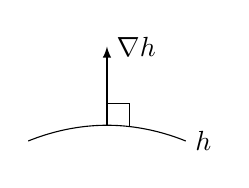
\begin{tikzpicture}
    \coordinate (u) at (1,0.2);
    \draw (0,0) parabola bend (u) (2,0) node [anchor=west] {$h$};
    \draw [->,>=latex] (u) -- ($(u)+(0,1)$) node [anchor=west] {$\nabla h$};
    \draw ($(u)+(0,8pt)$) coordinate (b) -- ($(b)!1!90:(u)$) coordinate (c);
    \draw [shorten >=-0.5pt] (c) -- ($(c)!1!90:(b)$);
  \end{tikzpicture}
\end{center}
We need $\nabla g \parallel \nabla h$ at $u^*$ for optimality, i.e.
\[ \pder{g}{u}(u^*) = \alpha \pder{h}{u}(u^*), \quad \text{for some } \alpha\in\R \]
or ($\lambda=-\alpha$),
\[ \pder{g}{u}(u^*) + \lambda \pder{h}{u}(u^*) = 0 \]
or
\[ \pder{}{u} \big( g(u^*) + \lambda h(u^*) \big) = 0, \quad \text{for some } \lambda\in\R \]
More generally,
\begin{align}
  \min_{u\in\mathcal R^m} {}\ & g(u) \\
  \text{s.t. } & h(u)=\bm 0, \quad h:\R^m\to\R^k
\end{align}
Note that $h(u)=[h_1(u),\dots,h_k(u)]\trans$.

We need $\pder{g}{u}(u^*)$ to be a linear combination of $\pder{h_i}{u}(u^*)$, $i=1,\dots,k$, for exactly the same reasons, i.e.
\[ \pder{g}{u}(u^*) = \sum_{i=1}^k \alpha_i \pder{h_i}{u}(u^*) \]
or ($\lambda=-[\alpha_1,\dots,\alpha_k]\trans$)
\[ \pder{g}{u}(u^*) + \lambda\trans \pder{h}{u}(u^*) = 0 \]
or
\[ \pder{}{u} \big( g(u^*) + \lambda\trans h(u^*) \big) = 0, \quad \text{for some } \lambda\in\R^k \]

\begin{thm}
  If $u^*$ is a minimizer to 
  \begin{align}
    \min_{u\in\mathcal R^m} {}\ & g(u) \\
    \text{s.t. } & h(u)=\bm 0, \quad h:\R^m\to\R^k
  \end{align}
  then $\exists\lambda\in\R^k$ s.t.
  \[ \begin{cases}
      \displaystyle \pder{L}{u}(u^*,\lambda) = 0 \\[2ex]
      \displaystyle \pder{L}{\lambda}(u^*,\lambda) = 0
    \end{cases} \]
  where the Lagrangian $L$ is given by
  \[ L(u,\lambda) = g(u) + \lambda\trans h(u) \]
\end{thm}

\paragraph{Note:}
\begin{itemize}
\item $\lambda$ are the Lagrange multipliers
\item $\pder{L}{\lambda}=0$ is fancy speak for $h(u^*)=0$
\end{itemize}

\paragraph{Example}
\begin{align}
  \min_{u\in\R^m} {}\ & \frac12 \Vert u\Vert^2 \\
  \text{s.t. } & Au=b
\end{align}
where $A$ is $k\times m$, $k\le m$. Assume $(AA\trans)^{-1}$ exists (constraints are linearly independent, none of the constraints are ``duplicates'', all the constraints are essential).
\begin{align}
  L &= \frac12 u\trans u + \lambda\trans (Au-b) \\
  \pder{L}{u} &= u\trans + \lambda\trans A = 0 \\
  u^* &= -A\trans \lambda \\
  \shortintertext{Using the equality constraint,}
  A u^* &= b \\
  -A A\trans \lambda &= b \\
  \lambda &= -(AA\trans)^{-1} b \\
  u^* &= A\trans (AA\trans)^{-1} b
\end{align}

\paragraph{Example}
\begin{align}
  \min {}\ & u_1u_2 + u_2u_3 + u_1u_3 \\
  \text{s.t. } & u_1 + u_2 + u_3 = 3
\end{align}
\[ L = u_1u_2 + u_2u_3 + u_1u_3 + \lambda (u_1 + u_2 + u_3 - 3) \]
\begin{align}
  \begin{cases}
    \pder{L}{u_1} = u_2 + u_3 + \lambda = 0 \\
    \pder{L}{u_2} = u_1 + u_3 + \lambda = 0 \\
    \pder{L}{u_3} = u_2 + u_1 + \lambda = 0 \\
    \pder{L}{\lambda} = u_1 + u_2 + u_3 = 3
  \end{cases}
  \Longrightarrow
  \begin{cases}
    u_1^* = 1 \\
    u_2^* = 1 \\
    u_3^* = 1 \\
    \lambda = -2
  \end{cases}
  \quad \text{optimal solution}
\end{align}
Note: This was actually the worst we can do---maximize! Even weirder: no local minimizer!

% 2017/01/19
\subsection{Equality Constraints}
\begin{align}
  \min_{u\in\mathcal R^m} {}\ & g(u) \\
  \text{s.t. } & h(u)=\bm 0, \quad h:\R^m\to\R^k
\end{align}
\begin{thm}
  If $u^*$ is a minimizer/maximizer then $\exists\lambda\in\R^k$ s.t.
  \begin{align}
    \pder{L}{u}(u^*,\lambda) &= 0 \\
    \pder{L}{\lambda}(u^*,\lambda) &= 0 \qquad (\Longleftrightarrow h(u^*)=0)
  \end{align}
  where $L(u,\lambda) = g(u) + \lambda\trans h(u)$.
\end{thm}

\paragraph{Example} [Entropy Maximization]

Given $S=\{x_1,\dots,x_n\}$ and a distribution over $S$ such that it takes the value $x_j$ with probability $p_j$. The entropy is
\[ E(p) = \sum_{j=1}^n (-p_j \ln p_j). \]
The mean is
\[ m = \sum_{j=1}^n p_jx_j. \]
Problem: Given $m$, find $p$ such that $E$ is maximized.
\begin{align}
  \min_{p} {}\ & -\sum_{j=1}^n p_j \ln p_j \\
  \text{s.t. } & \sum_{j=1}^n p_j x_j = m \\
               & \sum_{j=1}^n p_j = 1 \\
               & p_j \ge 0, \ j=1,\dots,n \quad \text{(ignore this\dots)}
\end{align}
\begin{align}
  L &= - \sum p_j \ln p_j + \lambda_1 \left[ \sum p_j x_j -m \right] + \lambda_2 \left[ \sum p_j - 1 \right] \\
  \pder{L}{p_j} &= -\ln p_j - 1 + \lambda_1 x_j + \lambda_2 = 0 \\
  p_j &= e^{\lambda_2 - 1 + \lambda_1 x_j}, \quad j=1,\dots,n \qquad (p_j\ge0 \text{ so we're ok with ignoring that})
\end{align}
\begin{align}
  \sum e^{\lambda_2 - 1 + \lambda_1 x_j} x_j &= m && n+2 \text{ equations and} \\
  \sum e^{\lambda_2 - 1 + \lambda_1 x_j} &= 1 && n+2 \text{ unknowns\dots}
\end{align}
No analytical solution, but numerically ``solvable''

\subsection{Inequality Constraints}
\begin{align}
  \min_{u\in\mathcal R^m} {}\ & g(u) \\
  \text{s.t. } & h(u)\le\bm 0, \quad h:\R^m\to\R^k
\end{align}
\begin{center}
  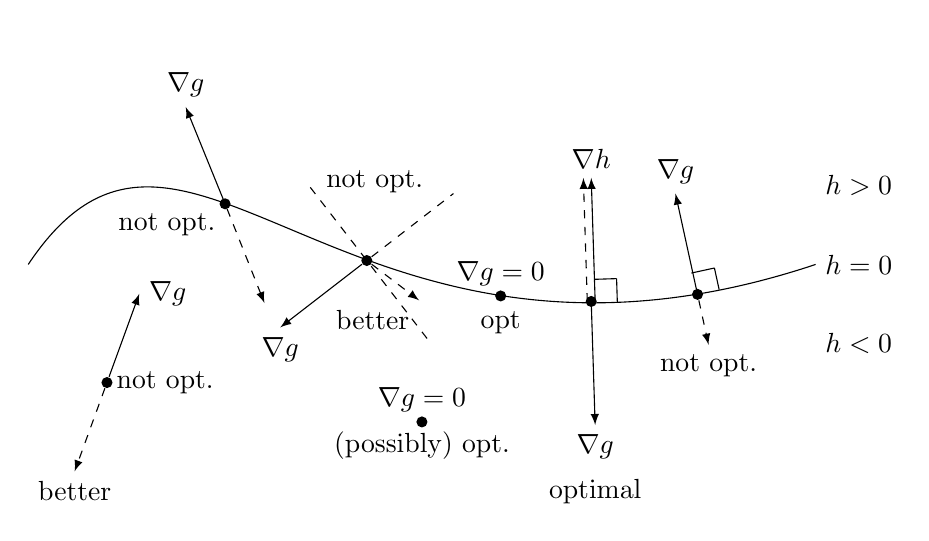
\begin{tikzpicture}[>=latex]
    \draw (0,0) .. controls (2,3) and (4,-2) .. (10,0) node [anchor=west] {$h=0$};
    \node [anchor=west] at (10,1) {$h>0$};
    \node [anchor=west] at (10,-1) {$h<0$};

    \path
    coordinate (u) at (2.5,0.77)
    coordinate  (A) at (2,2)
    coordinate (B) at (3,-0.49);
    \draw [->] (u) node [dot] {} -- (A) node [anchor=south] {$\nabla g$};
    \draw [<-,dashed] (B) -- (u) node [anchor=north east] {not opt.};

    \node [dot] (u3) at (6,-0.40) {};
    \node [anchor=south] at (u3) {$\nabla g=0$};
    \node [anchor=north,yshift=-2pt] at (u3) {opt};

    \coordinate (u2) at (7.2,-0.47);
    \coordinate (A2) at (7.15, 1.1);
    \draw [->] (u2) -- (A2) node [anchor=south] {$\nabla h$};
    \draw [->] ($(u2)+(-0.05,0)$) node [dot] {} -- ($(u2)!-1!(A2)+(-0.05,0)$) node [anchor=north] (D2) {$\nabla g$};
    \draw ($(u2)!8pt!(A2)$) coordinate (B2) -- ($(B2)!1!90:(u2)$) coordinate (C2);
    \draw [shorten >=-0.5pt] (C2) -- ($(C2)!1!90:(B2)$);
    \draw [->,dashed] ($(u2)+(-0.1,0)$) -- ($(A2)+(-0.1,0)$);
    \node [anchor=north,yshift=-8pt] at (D2) {optimal};

    \draw [->] (8.5,-0.38) node [dot] (u4) {} -- (8.22,0.9) coordinate (A4);
    \node [anchor=south] at (A4) {$\nabla g$};
    \draw [->,dashed] (u4) -- ($(u4)!-0.5!(A4)$) node [anchor=north] {not opt.};
    \draw [shorten <=-0.5pt] ($(u4)!8pt!(A4)$) coordinate (B4) -- ($(B4)!1!90:(u4)$) coordinate (C4);
    \draw (C4) -- ($(C4)!1!90:(B4)$);

    \node [dot] (u5) at (4.3,0.05) {};
    \draw [->] (u5) -- (3.2,-0.8) coordinate (a5);
    \node [anchor=north] at (a5) {$\nabla g$};
    \draw [dashed] (u5) -- ($(u5)!-1!(a5)$) coordinate (b5);
    \draw [dashed] ($(u5)!0.9!90:(a5)$) -- ($(u5)!0.9!90:(b5)$);
    \draw [->,dashed] (u5) -- ($(u5)!0.6!-75:(b5)$) node [anchor=north east] {better};
    \node at ($(u5)+(0.1,1)$) {not opt.};

    \node [dot] (u6) at (5,-2) {};
    \node [anchor=south] at (u6) {$\nabla g=0$};
    \node [anchor=north] at (u6) {(possibly) opt.};

    \node [dot] (u7) at (1,-1.5) {};
    \draw [->] (u7) -- +(70:1.2) coordinate (a7);
    \node [anchor=west] at (a7) {$\nabla g$};
    \draw [->,dashed] (u7) -- ($(u7)!-1!(a7)$) node [anchor=north] {better};
    \node [anchor=west] at (u7) {not opt.};
  \end{tikzpicture}
\end{center}

We need:
\begin{itemize}
\item if $h(u^*)<0$ then $\pder{g}{u}(u^*)=0$
\item if $h(u^*)=0$ then we need either
  \begin{gather}
    \pder{g}{u}(u^*) = 0 \\
    \shortintertext{or}
    \pder{g}{u}(u^*) = -\lambda\pder{h}{u}(u^*) \quad \text{for } \lambda>0
  \end{gather}
\end{itemize}
Or, even better,
\[ \pder{}{u} \left( g(u^*) + \lambda h(u^*) \right) = 0 \quad \text{for } \lambda\ge 0, \]
where $\lambda h(u^*)=0$. ($h<0\to\lambda=0$, $h=0\to\lambda\ge0$)

In general, if $u\in\R^m$ and $h:\R^m\to\R^k$, we have that $u^*$, if optimal, has to satisfy
\begin{gather}
  \pder{}{u} L(u^*,\lambda) = 0 \\
  h(u^*) \le \bm 0 \\
  \lambda\trans h(u^*) = 0 \\
  \lambda \ge \bm 0
\end{gather}
where the Lagrangian is $L(u,\lambda) = g(u) + \lambda\trans h(u)$. Note that if we're maximizing, the same holds except we need $\lambda\le 0$.

\paragraph{Example}
\begin{align}
  \min {}\ & 2u_1^2 + 2u_1u_2 + u_2^2 - 10u_1 - 10u_2 \\
  \text{s.t. } & \begin{cases}
    u_1^2 + u_2^2 \le 5 \\
    3u_1 + u_2 \le 6
  \end{cases}
\end{align}
\[ L = 2u_1^2 + 2u_1u_2 + u_2^2 - 10u_1 - 10u_2 + \lambda_1 (u_1^2 + u_2^2 - 5) + \lambda_2 (3u_1+u_2 - 6) \]
FONC:
\begin{enumerate}[label=\roman*)]
\item $\partial L/\partial u_1 = 4u_1 + 2u_2 - 10 + 2\lambda_1u_1 + 3\lambda_2$
\item $\partial L/\partial u_2 = 2u_1 + 2u_2 - 10 + 2\lambda_1u_2 + \lambda_2$
\item $u_1^2 + u_2^2 \le 5$
\item $3u_1 + u_2 \le 6$
\item $\lambda_1(u_1^2 + u_2^2 - 5) = 0$
\item $\lambda_2(3u_1 + u_2 - 6) = 0$
\item $\lambda_1 \ge 0$
\item $\lambda_2 \ge 0$
\end{enumerate}
To solve, assume different constraints are active/inactive:
\begin{enumerate}
\item Both constraints are inactive ($u_1^2 + u_2^2 < 5$, $3u_1 + u_2 < 6$) $\Longrightarrow \lambda_1=\lambda_2=0$
  \[ \begin{cases}
      4u_1 + 2u_2 - 10 = 0 \\
      2u_1 + 2u_2 - 10 = 0
    \end{cases}
    \Longrightarrow
    \begin{cases}
      u_1 = 0 \\
      u_2 = 5
    \end{cases} \]
  Note: iii) $0^2 + 5^2 \nleq 5$

  Not feasible

\item Assume constraint 1 is active and constraint 2 is inactive ($u_1^2 + u_2^2 = 5$, $\lambda_2=0$)
  \[ \begin{cases}
      4u_1 + 2u_2 - 10 + 2\lambda_1u_1 = 0 \\
      2u_1 + 2u_2 - 10 + 2\lambda_1u_2 = 0 \\
      u_1^2 + u_2^2 = 5
    \end{cases}
    \Longrightarrow
    \begin{cases}
      u_1 = 1 \\
      u_2 = 2 \\
      \lambda_1 = 1
    \end{cases} \]
  \begin{enumerate}[label=$\square$\hspace{1pt}\llap{\protect\raisebox{2pt}{$\checkmark$}}]
  \item $\lambda_1 \ge 0$
  \item $3\cdot 1 + 2 \le 6$
  \end{enumerate}
  This is a local minimizer

\item Assume constraint 2 is active and constraint 1 is inactive
\item Assume both constraints are active
\end{enumerate}

\paragraph{Kuhn-Tucker Conditions} (KKT conditions, Karush-Kuhn-Tucker)
\subparagraph{Problem:}
\begin{equation}
  \begin{aligned}
    \min_{u\in\R^m} {}\ & g(u) \\
    \text{s.t. } & \begin{cases}
      h_1(u) = 0, & h_1:\R^m\to\R^p \\
      h_2(u) \le 0, & h_2:\R^m\to\R^k
    \end{cases}
  \end{aligned}
  \label{eq:kkt}
\end{equation}

\begin{thm}
  Let $u^*$ be feasible ($h_1=0$, $h_2\le0$). If $u^*$ is a minimizer to \eqref{eq:kkt} than there exists vectors $\lambda\in\R^p$, $\mu\in\R^k$ with $\mu\ge\bm 0$ such that
  \[ \begin{cases}
      \displaystyle \pder{g}{u}(u^*) + \lambda\trans \pder{h_1}{u}(u^*) + \mu\trans \pder{h_2}{u}(u^*) = 0 \\[1ex]
      \mu\trans h_2(u^*) = 0
    \end{cases} \]
\end{thm}

Looking ahead: $\min \text{cost}(u(\cdot))$ s.t.\ $\dot x = f(x,u)$ (dynamics), where $u$ is a function. Note the equality constraint.

% 2017/01/24
\paragraph{Question:} How do we go from $u\in\R^m$ to $u\in\mathcal U$ (function space)?
\subparagraph{Note:} Function space is a set of functions of a given kind from a set $X$ to a set $Y$
\begin{enumerate}
\item linear function
\item square-integrable functions: $L_2[0,T]:$ $\int_0^T \Vert u(t)\Vert^2 \dif t < \infty$
\item $C^\infty (\R)$
\end{enumerate}
What would $\partial \text{``cost''}/\partial u$ mean?

\section{Directional Derivatives}
\paragraph{Recall:} To minimize $g(u)$, let $u^*$ be a candidate minimizer and pitch a perturbation on $u^*$ of $\varepsilon v$, where $\varepsilon$ is the scale and $v$ is the direction. Taking Taylor's expansion at the perturbation produces

\begin{center}
  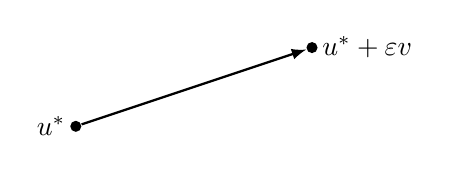
\begin{tikzpicture}
    \node [dot] (a) at (0,0) {};
    \node [dot] (b) at (3,1) {};
    \draw [>=latex,->,thick] (a) node [anchor=east] {$u^*$} -- (b) node [anchor=west] {$u^*+\varepsilon v$};
  \end{tikzpicture}
\end{center}

\begin{gather}
  g(u^* + \varepsilon v) = g(u^*) + \varepsilon \pder{g}{u}(u^*) v + o(\varepsilon) \\
  \text{FONC: } \pder{g}{u}(u^*) = 0 \hspace{3cm} 
\end{gather}

\subparagraph{Note:} $\pder{g}{u}(u^*) v$ tells us how much $g(u)$ increases/decreases in the direction of $v$.

\begin{defi}
  The directional (Gateaux) derivative is given by
  \[ \delta g(u;v) = \lim_{\varepsilon\to0} \frac{g(u+\varepsilon v)-g(u)}{\varepsilon} \]
\end{defi}

\paragraph{Example}
\[ g(u) = \frac12 u_1^2 - u_1 + 2u_2, \quad g:\R^2\to\R \]
Let's consider $e_1=[1\ 0]\trans$, $e_2=[0\ 1]\trans$. What is $\delta g(u;e_i)$, $i=1,2$?
\begin{align}
  \delta g(u;v) &= \lim_{\varepsilon\to0} \frac{g(u+\varepsilon v)-g(u)}{\varepsilon} \\
                &= \lim_{\varepsilon\to0} \frac{g(u)+\varepsilon\pder{g}{u}(u) v + o(\varepsilon) - g(u)}{\varepsilon} \\
                &= \pder{g}{u} (u) v
\end{align}
\begin{align}
  \pder{g}{u}(u) &= [u_1-1\ 2] \\
  \delta g(u;e_1) &= [u_1-1\ 2] e_1 = u_1-1 \\
  \delta g(u;e_2) &= [u_1-1\ 2] e_2 = 2 \\
\end{align}

But the beauty of directional derivatives is that they generalize beyond vectors, $u\in\R^m$, to function spaces ($\mathcal U$) or other ``objects'' like matrices.

\paragraph{Example} $M\in\R^{n\times n}$, $F(M)=M^2$

What is $\pder{F}{M}$? (ponder at home\dots)

We can easily compute $\delta F(M;N)$!
\begin{align}
  F(M+\varepsilon N) &= (M+\varepsilon N)(M+\varepsilon N) = M^2 + \varepsilon M N + \varepsilon N M + \varepsilon^2 N^2 \\
  \delta F(M;N) &= \lim_{\varepsilon\to0} \frac{F(M+\varepsilon N)-F(M)}{\varepsilon} \\
                  &= \lim_{\varepsilon\to0} \frac{\varepsilon M N + \varepsilon N M + \varepsilon^2 N^2}{\varepsilon} = MN + NM
\end{align}

\paragraph{Infinite Dimensional Optimization}
Let $u\in\mathcal U$ (function space) and let $J(u)$ be the cost:
\[ \min_{u\in\mathcal U} J(u) \]

\begin{thm}
  If $u^*\in\mathcal U$ is a (local) minimizer then
  \[ \delta J(u^*;v) = 0, \quad \forall v\in\mathcal U \]
\end{thm}

\paragraph{Example} Find minimizer $u^*$ to
\[ J(u) = \int_0^T L(u(t)) \dif t \]
\begin{align}
  J(u+\varepsilon v) - J(u) &= \int_0^T L(u(t)+\varepsilon v(t)) \dif t - \int_0^T L(u(t)) \dif t, \quad u,v\in\mathcal U \\
                         &= \int_0^T \left[ L(u(t)) + \varepsilon \pder{L}{u}(u(t)) v(t) + o(\varepsilon) - L(u(t)) \right] \dif t \\
  \delta J(u^*;v) &= \lim_{\varepsilon\to0} \frac{J(u+\varepsilon v)-J(u)}{\varepsilon} \\
                         &= \lim_{\varepsilon\to0} \frac{\int_0^T \varepsilon \pder{L}{u}(u(t)) v(t) \dif t + o(\varepsilon)}{\varepsilon} \\
                         &= \int_0^T \pder{L}{u}(u(t)) v(t) \dif t \\
\end{align}
$u^*$ optimizer:
\begin{gather}
  \delta J(u^*;v) = \int_0^T \pder{L}{u}(u(t)) v(t) \dif t = 0 \quad \forall v\in\mathcal U \\
  \Updownarrow \\
  \pder{L}{u} (u(t)) = 0 \quad \forall t\in[0,T]
\end{gather}
But, we want \emph{optimal control}! We want our cost to look like
\begin{gather}
  \int_0^T L(x(t),u(t)) \dif t \\
  \dot x = f(x,u)
\end{gather}

\section{Calculus of Variations}
What happens to $x(t)$ when $u(t)$ changes to $u(t)+\varepsilon v(t)$? Let the system be given by
\[ \begin{cases}
    \dot x = f(x,u) \\
    x(0) = x_0
  \end{cases} \]
After perturbation of $u$, the new system is
\[ \begin{cases}
    \dot{\hat x} = f(\hat x,u+\varepsilon v) \\
    x(0) = x_0
  \end{cases} \]

\pgfmathsetseed{11}
\begin{figure}
  \centering
  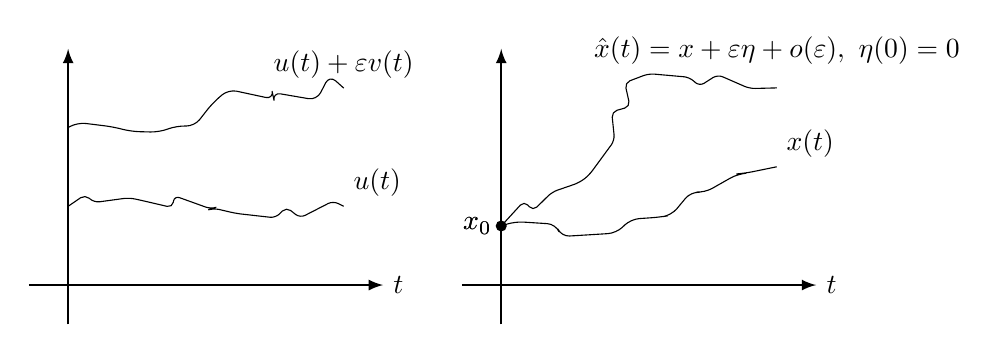
\begin{tikzpicture}
    \draw [thick,->] (-0.5,0) -- (4,0) node [anchor=west] {$t$};
    \draw [thick,->] (0,-0.5) -- (0,3) node [anchor=east] {};
    \draw [decorate, decoration={random steps, segment length=7pt, amplitude=5pt}, rounded corners=2pt] (0,1) to[in=180,out=0,distance=3.5cm] (3.5,1) node [anchor=south west] {$u(t)$};
    \draw [decorate, decoration={random steps, segment length=8pt, amplitude=5pt}, rounded corners=3pt] (0,2) to[in=180,out=0,distance=3cm] (3.5,2.5) node [anchor=south] {$u(t)+\varepsilon v(t)$};

    \draw [thick,->] (5,0) -- (9.5,0) node [anchor=west] {$t$};
    \draw [thick,->] (5.5,-0.5) -- (5.5,3) node [anchor=east] {};
    \draw [decorate, decoration={random steps, segment length=8pt, amplitude=4pt}, rounded corners=3pt] (5.5,0.75) node [anchor=east] {$x_0$} to[in=200,out=0,distance=3cm] (9,1.5) node [anchor=south west] {$x(t)$};
    \draw [decorate, decoration={random steps, segment length=8pt, amplitude=5pt}, rounded corners=2pt] (5.5,0.75) node [anchor=east] {$x_0$} to[in=170,out=30,distance=3cm] (9,2.5) node [anchor=south,yshift=5pt] {$\hat x(t)=x+\varepsilon\eta+o(\varepsilon),\ \eta(0)=0$};
    \node [dot] at (5.5,0.75) {};
  \end{tikzpicture}
  \caption{Variation in $u$ causes a variation in $x$.}
  \label{fig:var_u_x}
\end{figure}

\noindent
Consider
\[ \tilde x=x+\varepsilon \eta, \]
where
\begin{alignat}{2}
  \dot x&=f(x,u), & x(0) &= x_0 \\
  \dot \eta &= \pder{f}{x}(x,u) \eta + \pder{f}{u}(x,u) v, \qquad & \eta(0) &= 0
\end{alignat}

\begin{thm}
  If $f$ is continuously differentiable in $x$ and $u$ then
  \[ \hat x(t) = \tilde x(t) + o(\varepsilon) \]
  \begin{proof}
    \mbox{}
    \begin{enumerate}[label=\roman*)]
    \item Initial conditions:
      \begin{align}
        \hat x(0) &= x_0 \\
        \tilde x(0) &= x(0) + \varepsilon \eta(0) = x_0
      \end{align}
    \item Dynamics:
      \begin{align}
        \dot{\hat x} &= f(\hat x,u+\varepsilon v) \\
        \dot{\tilde x} &= \dot x + \varepsilon \dot \eta = f(x,u) + \varepsilon \pder{f}{x}(x,u)\eta + \varepsilon \pder{f}{u}(x,u) v \\
                     &= f(x+\varepsilon\eta,u+\varepsilon v) + o(\varepsilon) \\
                     &= f(\tilde x,u+\varepsilon v) + o(\varepsilon)
      \end{align}
      We can see that the dynamics of $\hat x(t)$ are equal to those of $\tilde x(t)$ plus higher order terms:
      \begin{align}
        \dot{\tilde x} &= f(\tilde x,u+\varepsilon v) + o(\varepsilon) \\
        \dot{\hat x} &= f(\hat x,u+\varepsilon v)
      \end{align}
      Therefore, if our perturbation is small enough, we can model $\hat x(t)$ as $\tilde x(t)$.
    \end{enumerate}
  \end{proof}
\end{thm}

\begin{framed}
  \hypertarget{taylor_2var}{}
  Note: Taylor expansion with two elements is
  \begin{align}
    h(w+\varepsilon v,z+\varepsilon y) &= h(w,z+\varepsilon y) + \pder{h}{w}(w,z+\varepsilon y)\varepsilon v + o(\varepsilon) \\
                                       &= \left\{ h(w,z) + \pder{h}{z}(w,z)\varepsilon y + o(\varepsilon) \right\} \\
                                       & \qquad + \left\{ \pder{h}{w}(w,z)\varepsilon v + \underbrace{\pder{^2 h}{z\partial w}\varepsilon v \odot \varepsilon y}_{o(\varepsilon)} + o(\varepsilon) \right\} \\
                                       &= h(w,z) + \pder{h}{z}\varepsilon y + \pder{h}{w}\varepsilon v + o(\varepsilon)
  \end{align}
\end{framed}

% 2017/01/26
\paragraph{Last class:} \mbox{}
\begin{enumerate}
\item $u\in\U$ (space of functions), $J:\U\to\R$ (cost).

  FONC: If $u^*$ is optimal, then
  \[ \delta J(u;\nu) = 0 \quad \forall \nu\in\U, \]
  where the directional derivative is given by
  \[ \delta J(u;\nu) = \lim_{\varepsilon\to0} \frac{J(u+\varepsilon \nu)-J(u)}{\varepsilon}. \]
\item If
  \[ \begin{cases}
      \dot x = f(x,u) \\
      x(0) = x_0
    \end{cases} \]
  then a variation in $u$:
  \[ u \longmapsto u+\varepsilon \nu \]
  results in a variation in $x$:
  \[ x \longmapsto x+\varepsilon\eta + o(\varepsilon) \]
  See \autoref{fig:var_u_x}. Note $\eta(0)=0$.
\end{enumerate}

\subsection{An (Almost) Optimal Control Problem}

Let $\dot x=f(x)$, $x(0)=x_0$. Note we get to pick the initial condition!
\subparagraph{Problem}
\begin{gather}
  \min_{x_0\in\R^m} J(x_0) = \int_0^T L(x(t)) \dif t \\
  \text{s.t. } \begin{cases}
    \dot x(t) = f(x(t)) & \text{the \emph{constraint}! (equality)} \\
    x(0)=x_0
  \end{cases}
\end{gather}
Note every constraint needs a Lagrange multiplier. We have infinitely many constraints:
\[ \dot x(t) = f(x(t)) \quad \forall t\in[0,T] \]
We need $\lambda(t)$ as a function of $t$. Also, the sum in the Lagrangian has to become an integral. The continuous-time Lagrangian thus becomes
\[ \tilde J(x_0,\lambda) = \int_0^T \Big[ L(x(t)) + \lambda\trans(t) (f(x(t))-\dot x(t)) \Big] \dif t \]
The task is to perturb $x_0$ as $x_0\longmapsto x_0+\varepsilon \nu$, $\nu\in\R^m$ and compute
\[ \delta \tilde J(x_0;\nu) = \lim_{\varepsilon\to0} \frac{\tilde J(x_0+\varepsilon \nu)-\tilde J(x_0)}{\varepsilon} \]
and make this equal to 0 $\forall \nu\in\R^m$. The variation in $x$ is

\pgfmathsetseed{11}
\begin{center}
  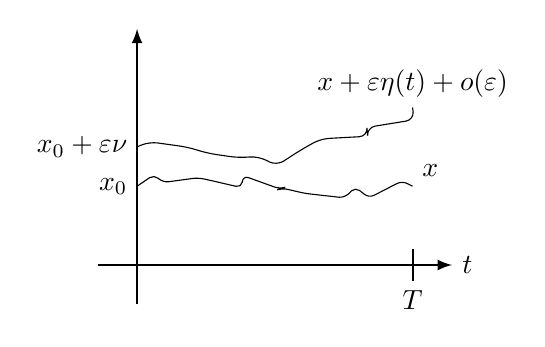
\begin{tikzpicture}
    \draw [->,thick] (-0.5,0) -- (4,0) node [anchor=west] {$t$};
    \draw [->,thick] (0,-0.5) -- (0,3);
    \draw [decorate, decoration={random steps, segment length=7pt, amplitude=5pt}, rounded corners=2pt] (0,1) node [anchor=east] {$x_0$} to[in=180,out=0,distance=3.5cm] (3.5,1) node [anchor=south west] {$x$};
    \draw [decorate, decoration={random steps, segment length=9pt, amplitude=5pt}, rounded corners=3pt] (0,1.5) node [anchor=east] {$x_0+\varepsilon \nu$} to[in=200,out=0,distance=3.5cm] (3.5,2) node [anchor=south] {$x+\varepsilon\eta(t)+o(\varepsilon)$};
    \draw [thick] (3.5,0.2) -- (3.5,-0.2) node [anchor=north] {$T$};
  \end{tikzpicture}
\end{center}

Note:

\hspace{\parindent}
\begin{tabular}{cl}
  $x_0$ & decision variable \\
  $\eta$ & variation in $x_0$ \\
  $x(t)$ & trajectory starting at $x_0$ \\
  $\eta(t)$ & change in trajectory resulting from $\nu$-variation in $x_0$ \\
  $\lambda(t)$ & time-varying Lagrange multiplier
\end{tabular}

\begin{align}
  \tilde J(x_0+\varepsilon \nu) &= \int_0^T \Big\{ L(x(t)) + \lambda\trans(t) [f(x(t)+\varepsilon\eta(t)) - \dot x(t) - \varepsilon\dot\eta(t)] \Big\} \dif t + o(\varepsilon) \\
                           &= \int_0^T \left[ L(x) + \varepsilon\pder{L}{x}(x)\eta + \lambda\trans \left( f(x) + \varepsilon\pder{f}{x}(x)\eta - \dot x - \varepsilon\dot\eta \right) \right] \dif t + o(\varepsilon) \\
  \tilde J(x_0+\varepsilon \nu) - \tilde J(x_0) &= \int_0^T \left[ \varepsilon\pder{L}{x}(x)\eta + \lambda\trans\left( \varepsilon\pder{f}{x}\eta - \varepsilon\dot\eta \right) \right] \dif t + o(\varepsilon) \\
  \delta \tilde J (x_0;\nu) &= \int_0^T \left[ \pder{L}{x}(x)\eta + \lambda\trans\left( \pder{f}{x}\eta - \dot\eta \right) \right] \dif t
\end{align}
A powerful idea: we want $\delta\tilde J(x_0;\nu)=0$ $\forall \nu$. Somehow get this in the form
\[ \int_0^T \Big(\text{stuff}(t)\Big) \eta(t) \dif t = 0 \]
We can pick $\text{stuff}(t)=0$ $\forall t\in[0,T]$.

In $\delta\tilde J(x_0;\nu)$ we have $\dot\eta$ (problem!). We can solve this using \emph{integration by parts}.
\[ \int_0^T \lambda\trans \dot\eta \dif t = \lambda\trans(T)\eta(T) - \lambda\trans(0)\eta(0) - \int_0^T \dot\lambda\trans\eta \dif t \]
Hence,
\[
  \delta\tilde J(x_0;\nu) = \int_0^T \underbrace{\big( \pder{L}{x} + \lambda\trans\pder{f}{x} + \dot\lambda\trans \big)}_{\text{pick}=0} \eta \dif t - \underbrace{\lambda\trans(T)}_{\text{pick}=0} \eta(T) + \lambda\trans(0) \underbrace{\eta(0)}_{\nu}
\]
We are free to pick $\lambda$ freely if it gives $\delta\tilde J=0$.
\[ \text{Pick: } \begin{cases}
    \dot\lambda(t) = -\pder{L\trans}{x}(x(t)) - \pder{f\trans}{x}(x(t)) \lambda(t) \\
    \lambda(T) = 0 & \text{backwards diff. eq:}
  \end{cases} \]
Under this choice of $\lambda$ we get
\[ \delta\tilde J(x_0;\nu) = \lambda\trans(0) \nu \]
This is linear in $\nu$ so the FONC is $\lambda(0)=0$.

Moreover, we really have a ``normal'' optimization problem
\begin{gather}
  \min_{x_0\in\R^m} \tilde J(x_0) \\
  \delta \tilde J(x_0;\nu) = \pder{\tilde J}{x_0} (x_0) \nu
\end{gather}
which means that
\[ \pder{\tilde J}{x_0} = \lambda\trans(0) \]
If $x_0^*$ minimizes
\begin{gather}
  \int_0^T L(x(t)) \dif t \\
  \text{s.t. } \begin{cases}
    \dot x(t) = f(x(t)) \\
    x(0) = x_0^*
  \end{cases}
\end{gather}
then
\[ \lambda(0) = \bm 0 \]
where $\lambda(t)$ satisfies
\[ \begin{cases}
    \dot \lambda(t) = -\pder{L\trans}{x}(x(t)) - \pder{f\trans}{x}(x(t)) \lambda(t) \\
    \lambda(T) = 0
  \end{cases} \]

\paragraph{So what?} We actually have a two-point boundary value problem. 
\begin{align}
  \dot x &= f(x) & \dot\lambda &= -\pder{L\trans}{x} - \pder{f\trans}{x} \lambda \\
  x(0) &= x_0 & \lambda(T) &= 0
\end{align}

\begin{center}
  \begin{tikzpicture}
    \draw [thick,->] (0,0) -- (4,0) node [anchor=west] {$t$};
    \draw [thick,->] (0,0) -- (0,3);
    \draw (-0.2,1.5) node [anchor=east] {$x_0$} -- (0.2,1.5);
    \draw [->,>={Straight Barb[scale length=2]}] (0,1.5) parabola bend (0.6,2) (1.5,1.5);
    \draw (1.5,1.5) parabola bend (2,1.3) (3.5,2.5);

    \draw [thick,->] (6,0) -- (10,0) node [anchor=west] {$t$};
    \draw [thick,->] (6,0) -- (6,3);
    \draw (9.5,0.2) -- (9.5,-0.2) node [anchor=north] {$T$};
    \draw [-{Straight Barb[scale length=2]}] (9.5,0) .. controls (8.25,0) and (9,1.5) .. (8,1.5) node [anchor=south] {$\lambda$};
    \draw (8,1.5) .. controls (7,1.25) .. (6,1.5);
    \draw (6.2,1.5) -- (5.8,1.5) node [anchor=east] {$\lambda(0)$};
  \end{tikzpicture}
\end{center}
We want to find $x_0$ that gives $f(x)$ such that after solving backwards for $\lambda(t)$, we find that
\[ \lambda(0) = \pder{\tilde J\trans}{x_0} = 0. \]
This leads to the following:

\paragraph{An algorithm} \mbox{}

\begin{algorithm}
  \begin{algorithmic}
    \State Pick $x_{0,0}$
    \State $k=1$
    \Repeat
    \State Simulate $x(t)$ from $x_{0,k}$ over $[0,T]$
    \State Simulate $\lambda(t)$ from $\lambda(T)=0$ backwards using $x(t)$
    \State Update $x_{0,k}$ as
    $ x_{0,k+1} = x_{0,k} - \gamma\lambda(0) $ \Comment{$\lambda(0)$ is the gradient}
    \State $k\coloneqq k+1$
    \Until $\lambda(0)=0$
  \end{algorithmic}
\end{algorithm}

\paragraph{Example:} \texttt{optinit.m}

\[ \dot x = Ax, \quad L=x\trans Qx-q, \quad Q=Q\trans \succ 0 \]
\vspace{-2em}
\begin{align}
  \dot \lambda &= -2Qx - A\trans\lambda \\
  \lambda(0) &= 0
\end{align}

% 2017/01/31
\subsection{Optimal Timing Control}
When to switch between modes?
\begin{equation}
  \begin{aligned}
    \dot x &= \begin{cases}
      f_1(x) & \text{if } t\in[0,\tau) \\
      f_2(x) & \text{if } t\in[\tau,T]
    \end{cases} \\
    x(0) &= x_0
  \end{aligned} \label{eq:otc}
\end{equation}

\begin{center}
  \begin{tikzpicture}
    \draw [->,thick] (-0.2,0) -- (5.5,0) node [anchor=west] {$t$};
    \draw [->,thick] (0,-0.2) -- (0,3.2);
    \draw (4.8,0.2) -- (4.8,-0.2) node [anchor=north] {$T$};
    \draw (2.2,0.2) -- (2.2,-0.2) node [anchor=north] {$\tau$};
    \draw (0.2,1) -- (-0.2,1) node [anchor=east] {$x_0$};
    \draw (0,1) parabola (2.2,2.8);
    \draw (2.2,2.8) parabola [bend at end] (4.8,1.2) node [anchor=west] {$x$};
    \node at (1,1.8) {$f_1$};
    \node at (4,1.8) {$f_2$};
  \end{tikzpicture}
\end{center}

\begin{align}
  & \min_\tau \int_0^T L(x(t)) \dif t = J(\tau) \\
  & \text{s.t.~\eqref{eq:otc} holds}
\end{align}

\begin{enumerate}[label=Step \arabic*:]
\item Augment cost with constraint
  \[ \tilde J = \int_0^\tau \Big[ L(x) + \lambda\trans(f_1(x)-\dot x) \Big] \dif t + \int_\tau^T \Big[ L(x) + \lambda\trans(f_2(x)-\dot x) \Big] \dif t \]
\item Variation $\tau\longmapsto\tau+\varepsilon\theta$
  \begin{center}
    \begin{tikzpicture}
      \draw [->,thick] (-0.2,0) -- (5.5,0) node [anchor=west] {$t$};
      \draw [->,thick] (0,-0.2) -- (0,3.2);
      \draw (4.8,0.2) -- (4.8,-0.2) node [anchor=north] {$T$};
      \draw (2.2,0.2) -- (2.2,-0.2) node [anchor=north] {$\tau$};
      \draw (3,0.2) -- (3,-0.2) node [anchor=north,yshift=3pt] {$\tau+\varepsilon\theta$};
      \draw (0.2,1) -- (-0.2,1) node [anchor=east] {$x_0$};
      \draw (0,1) parabola (2.2,1.8);
      \draw (2.2,1.8) parabola [bend at end] (4.8,1.2) node [anchor=west] {$x$};
      \node at (1,1.8) {$f_1$};
      \node at (3.6,1.7) {$f_2$};

      \begin{scope}
        \clip (4.8,4) rectangle (2.2,1.8);
        \draw [dashed] (2.2,1.8) parabola bend (0,1) (3,2.5);
        \draw [dashed] (3,2.5) parabola [bend at end] (5.4,1.9);
      \end{scope}
      \node [anchor=west] at (4.8,1.9) {$x+\varepsilon\eta+o(\varepsilon)$};
      \node at (2.4,2.4) {$f_1$};
      \node at (3.9,2.5) {$f_2$};
    \end{tikzpicture}
  \end{center}
\item Compute $\delta\tilde J(\tau;\theta)$
\end{enumerate}
\begin{align}
  \tilde J(\tau+\varepsilon\theta) &= \int_0^{\tau+\varepsilon\theta} \Big\{ L(x+\varepsilon\eta) + \lambda\trans[f_1(x+\varepsilon\eta)-\dot x-\varepsilon\dot\eta] \Big\} \dif t \\
                                & \qquad + \int_{\tau+\varepsilon\theta}^T \Big\{ L(x+\varepsilon\eta) + \lambda\trans[f_2(x+\varepsilon\eta)-\dot x-\varepsilon\dot\eta] \Big\} \dif t + o(\varepsilon) \\
  \intertext{Note that $\eta=\dot\eta=0$ on $[0,\tau)$.}
  \tilde J(\tau+\varepsilon\theta) &= \int_0^\tau \Big\{ L(x) + \lambda\trans[f_1(x)-\dot x] \Big\} \dif t \\
                                & \qquad + \int_\tau^{\tau+\varepsilon\theta} \Big\{ \underbrace{L(x+\varepsilon\eta)}_{L(x)+\varepsilon\pder{L}{x}\eta} + \lambda\trans[\underbrace{f_1(x+\varepsilon\eta)}_{f_1(x)+\varepsilon\pder{f_1}{x}\eta} - \dot x-\varepsilon\dot\eta] \Big\} \dif t \\
                                & \qquad + \int_{\tau+\varepsilon\theta}^T \Big\{ \underbrace{L(x+\varepsilon\eta)}_{L(x)+\varepsilon\pder{L}{x}\eta} + \lambda\trans[\underbrace{f_2(x+\varepsilon\eta)}_{f_2(x)+\varepsilon\pder{f_2}{x}\eta} - \dot x-\varepsilon\dot\eta] \Big\} \dif t + o(\varepsilon) \displaybreak \\
  \delta\tilde J(\tau;\theta) &= \lim_{\varepsilon\to0} \frac{\tilde J(\tau+\varepsilon\theta) - \tilde J(\tau)}{\varepsilon} \\
  \tilde J(\tau+\varepsilon\theta) - \tilde J(\tau) &= \int_0^\tau 0\cdot\dif t + \underbrace{ \int_\tau^{\tau+\varepsilon\theta} \left[ \varepsilon\pder{L}{x}\eta + \lambda\trans \Big(f_1(x)+\varepsilon\pder{f_1}{x}\eta - f_2(x) - \varepsilon\dot\eta \Big) \right] \dif t }_{\displaystyle I_1} \\
                                & \qquad + \underbrace{ \int_{\tau+\varepsilon\theta}^T \left[ \varepsilon\pder{L}{x}\eta + \lambda\trans \Big( \varepsilon\pder{f_2}{x}\eta - \varepsilon\dot\eta \Big) \right] \dif t }_{\displaystyle I_2} + o(\varepsilon)
\end{align}

\begin{framed}
\begin{thm}[Mean-value theorem]
  \[ \int_{t_1}^{t_2} h(t) \dif t = (t_2-t_1) h(\xi) \quad \text{for some}\ \xi\in[t_1,t_2] \]
\end{thm}
\end{framed}

\noindent
The first integral is
\begin{align}
  I_1 &= \int_\tau^{\tau+\varepsilon\theta} \left[ \varepsilon\pder{L}{x}\eta + \lambda\trans (f_1(x)+\varepsilon\pder{f_1}{x}\eta-\varepsilon\dot\eta-f_x(x)) \right] \dif t \\
  &= \varepsilon\theta \Big\{ \lambda\trans(\xi) \big[ f_1(x(\xi)) - f_2(x(\xi)) \big] \Big\} + o(\varepsilon)
\end{align}
Note that as $\varepsilon\to0$, $\xi\to\tau$. Using integration by parts, the second integral is
\begin{align}
  \int_\tau^T \lambda\trans \dot\eta \dif t &= \lambda\trans(T) \eta(T) - \lambda\trans(\tau) \underbrace{\eta(\tau)}_{=0} - \int_\tau^T \dot\lambda\trans \eta \dif t \\
  I_2 &= \int_\tau^T \left[ \varepsilon\pder{L}{x}\eta + \lambda\trans \Big( \varepsilon\pder{f_2}{x}\eta - \varepsilon\dot\eta \Big) \right] \dif t - \underbrace{ \int_\tau^{\tau+\varepsilon\theta} \left[ \varepsilon\pder{L}{x}\eta + \lambda\trans \Big( \varepsilon\pder{f_2}{x}\eta - \varepsilon\dot\eta \Big) \right] \dif t }_{o(\varepsilon)} \\
                                            &= \varepsilon \int_\tau^T \left[ \pder{L}{x} + \lambda\trans \pder{f_2}{x} + \dot\lambda\trans \right] \eta \dif t - \varepsilon \lambda\trans(T)\eta(T) + o(\varepsilon)
\end{align}
Hence,
\begin{align}
  \delta\tilde J(\tau;\theta) &= \lim_{\varepsilon\to0} \frac{\tilde J(\tau+\varepsilon\theta) - \tilde J(\tau)}{\varepsilon} \\
                              &= \theta\lambda\trans(\tau) \Big[ f_1(x(\tau)) - f_2(x(\tau)) \Big] + \int_\tau^T \left[ \pder{L}{x} + \lambda\trans \pder{f_2}{x} + \dot\lambda\trans \right] \eta \dif t - \lambda\trans(T)\eta(T)
\end{align}

\begin{enumerate}[resume*]
\item Select the \emph{costate} $\lambda(t)$. The key idea is to get rid of any term that has $\eta$ in it, i.e.
  \begin{align}
    \dot\lambda &= -\pder{L\trans}{x} - \pder{f_2\trans}{x} \lambda \quad \text{on } [\tau,T] \\
    \lambda(T) &= 0
  \end{align}
\item With this choice of $\lambda(t)$, we have
  \[ \delta\tilde J(\tau;\theta) = \theta\lambda\trans(\tau) \Big[ f_1(x(\tau)) - f_2(x(\tau)) \Big] = \pder{\tilde J}{\tau} \theta. \]
  Therefore,
  \[ \pder{\tilde J}{\tau} = \lambda\trans(\tau) \Big[ f_1(x(\tau)) - f_2(x(\tau)) \Big] = 0 \quad \text{(for optimality)} \]
\end{enumerate}

\paragraph{Algorithm} \mbox{}
\begin{algorithm}
  \begin{algorithmic}
    \State Pick $\tau_0$
    \State $k=0$
    \Repeat
    \State Simulate $x$ forward in time from $x(0)=x_0$
    \State Simulate $\lambda$ backwards from $\lambda(T)=0$
    \State Update $\tau_k$ as
    $ \tau_{k+1} = \tau_k - \gamma\lambda\trans(\tau_k) \big[ f_1(x(\tau_k)) - f_2(x(\tau_k)) \big] $
    \State $k\coloneqq k+1$
    \Until $\Vert \lambda\trans(f_1-f_2) \Vert < \varepsilon$
  \end{algorithmic}
\end{algorithm}

Where are we going? Come up with general principles for $\min_{u\in\mathcal U} J(u)$:
\begin{itemize}
\item Costate equations
\item Optimality conditions
\item Algorithms
\item Applications
\end{itemize}

% 2017/02/02
\subsection{The Bolza Problem}
Up until now, we have optimized with respect to finite-dimensional parameters. Today, we will minimize with respect to $u\in\mathcal U$.

\begin{align}
  & \min_{u\in\mathcal U} J(u) = \int_0^T L(x(t),u(t),t) \dif t + \underbrace{\Psi(x(T))}_{\substack{\text{terminal cost}\\ \text{(parking cost)}}} \\
  & \begin{aligned}
    \text{s.t.}\quad \dot x(t) &= f(x(t),u(t),t) \\
    x(0) &= x_0
  \end{aligned}
\end{align}
Assume that $f$ and $L$ are $C^1$ in $x,u$ and piecewise continuous in $t$. Then, a small change in $u$ causes small changes in $f$ and $L$. The variation: $u\longmapsto u+\varepsilon v$, $\varepsilon\in\R$, $v\in\mathcal U$. See \autoref{fig:var_u_x}.
\begin{align}
  \tilde J(u) &= \int_0^T \left[ L(x,u,t) + \lambda\trans (f(x,u,t)-\dot x) \right] \dif t + \Psi(x(T)) \\
  \tilde J(u+\varepsilon v) &= \int_0^T \left[ L(x+\varepsilon\eta,u+\varepsilon v, t) + \lambda\trans(f(x+\varepsilon\eta,u+\varepsilon v, t) - \dot x - \varepsilon\dot\eta) \right] \dif t \\
              & \qquad + \Psi(x(T)+\varepsilon\eta(T)) + o(\varepsilon) \\
  \tilde J(u+\varepsilon v) - \tilde J(u) &= \int_0^T \bigg[ L(x+\varepsilon\eta,u+\varepsilon v,t) - L(x,u,t) \\
              & \qquad\qquad + \lambda\trans\Big( f(x+\varepsilon\eta,u+\varepsilon v,t) - f(x,u,t) - \dot x - \varepsilon\dot\eta + \dot x \Big) \bigg] \dif t \\
              & \qquad + \Psi(x(T)+\varepsilon\eta(T)) - \Psi(x(T)) + o(\varepsilon) \\
              &= \int_0^T \left[ \pder{L}{x}\varepsilon\eta + \pder{L}{u}\varepsilon v + \lambda\trans\bigg( \pder{f}{x}\varepsilon\eta + \pder{f}{u}\varepsilon v - \varepsilon\dot\eta \bigg) \right] \dif t \\
              & \qquad + \pder{\Psi}{x}(x(T))\varepsilon\eta(T) + o(\varepsilon) \\
  \shortintertext{(See \hyperlink{taylor_2var}{Taylor expansion with respect to two variables}.)}
  \delta\tilde J(u;v) &= \int_0^T \left(\pder{L}{u} + \lambda\trans\pder{f}{u}\right)v\dif t + \int_0^T \left[\left(\pder{L}{x} + \lambda\trans\pder{f}{x}\right)\eta - \lambda\trans\dot\eta\right] \dif t \\
              & \qquad + \pder{\Psi}{x}(x(T))\eta(T) \\
  \shortintertext{Integrating by parts,}
  \int_0^T \lambda\trans\dot\eta\dif t &= \lambda\trans(T)\eta(T) - \lambda\trans(0)\eta(0) - \int_0^T \dot\lambda\trans\eta \dif t \\
              &= \lambda\trans(T)\eta(T) - \int_0^T \dot\lambda\trans\eta \dif t \\
  \delta\tilde J(u;v) &= \int_0^T \left(\pder{L}{u}+\lambda\trans\pder{f}{u}\right) v\dif t + \int_0^T \left(\pder{L}{x}+\lambda\trans\pder{f}{x} + \dot\lambda\trans\right)\eta \dif t \\
              & \qquad + \left(\pder{\Psi}{x}(x(T))-\lambda\trans(T)\right)\eta(T) \\
  \intertext{For optimality, we need the directional derivative to be zero for every $v\in\mathcal U$, where $v$ represents the direction of the derivative. Therefore, the term $(\pder{L}{u}+\lambda\trans\pder{f}{u})$ in the first integral has to be identically zero. Thus, we need}
  & \begin{dcases}
    \pder{L}{u} + \lambda\trans\pder{f}{u} = 0, & \forall t\in[0,T] \\
    \pder{L}{x} + \lambda\trans\pder{f}{x} + \dot\lambda\trans = 0, & \forall t\in[0,T] \\
    \pder{\Psi}{x}(x(T)) - \lambda\trans(T) = 0
  \end{dcases}
\end{align}
\begin{framed}
  \begin{defi}
    Let the \emph{Hamiltonian} $H(x,u,t,\lambda)$ be given by
    \[ H(x,u,t,\lambda) = L(x,u,t) + \lambda\trans f(x,u,t) \]
  \end{defi}
\end{framed}
\begin{thm}
  For $u$ to solve the Bolza problem, it has to satisfy
  \[ \pder{H}{u}(x,u,t,\lambda) = 0, \]
  where the \emph{costate} satisfies
  \[ \begin{dcases}
    \dot\lambda = - \pder{H\trans}{x}(x,u,t,\lambda) \\
    \lambda(T) = \pder{\Psi\trans}{x}(x(T))
  \end{dcases} \]
\end{thm}

\paragraph{Example} \mbox{}
\begin{align}
  & \min_u \int_0^1 \frac12 u^2(t) \dif t + \frac12 x^2(1) \\
  & \text{s.t. } \begin{cases}
    \dot x = u, & x,u\in\R \\
    x(0) = 1
  \end{cases}
\end{align}
\begin{align}
  H &= \frac12 u^2 + \lambda u \\
  \pder{H}{u} &= u + \lambda = 0 \Longrightarrow u=-\lambda \\
  \dot\lambda &= -\pder{H}{x} = 0 \Longrightarrow \lambda(t) = c \\
  \lambda(T) &= c = \pder{\Psi}{x}(x(1)) = x(1) \\
  \dot x &= u = -c \Longrightarrow x(t) = -ct + x(0) = -ct + 1 \\
  x(1) &= -c + 1 \\
  \lambda(1) &= c = x(1) = -c + 1 \Longrightarrow c = \frac12 \\
  \Aboxed{u^* &= -\frac12}
\end{align}
\begin{center}
  \begin{tikzpicture}
    \draw [thick,->] (-0.5,0) -- (4,0) node [anchor=west] {$t$};
    \draw [thick,->] (-0.5,5) -- (4,5) node [anchor=west] {$t$};
    \draw [thick,->] (0,3.5) -- (0,6) node [anchor=south] {$u$};
    \draw [thick,->] (0,-1) -- (0,2.5) node [anchor=south] {$x$};

    \draw (-0.2,4) node [anchor=east] {$-\dfrac12$} -- (3.5,4);
    \draw (3.5,4.8) -- (3.5,5.2) node [anchor=south] {$1$};

    \draw (-0.2,2) node [anchor=east] {$1$} -- (0.2,2);
    \draw (-0.2,1) node [anchor=east] {$\dfrac12$} -- (0.2,1);
    \draw (3.5,-0.2) node [anchor=north] {$1$} -- (3.5,0.2);
    \draw (0,2) -- (3.5,1);
  \end{tikzpicture}
\end{center}

We really used five different equations to solve this!
\begin{enumerate}[label=\roman*)]
\item $\displaystyle \pder{H}{u} = 0$
\item $\displaystyle \dot\lambda = - \pder{H\trans}{x}$
\item $\displaystyle \lambda(T) = \pder{\Psi\trans}{x}(x(T))$
\item $\dot x = f(x,u,t)$
\item $x(0) = x_0$
\end{enumerate}
There is a sixth condition that is pretty useful if $L$ and $f$ do not depend on $t$ ($L(x,u)$, $f(x,u)$). This is called a \emph{conservative system}. Then, along optimal trajectories (equations i-v are satisfied), the total time derivative of the Hamiltonian is
\[
  \frac{\dif}{\dif t} H = \underbrace{\pder{H}{t}}_{\mathclap{\substack{0\\ H(x,u,\lambda)}}} + \underbrace{\pder{H}{x}}_{-\dot\lambda\trans} \dot x + \underbrace{\pder{H}{u}}_{\mathclap{\substack{0\\ \text{ $u$ is optimal}}}} \dot u + \underbrace{\pder{H}{\lambda}}_{\mathclap{f\trans=\dot x\trans}} \dot\lambda
  = -\dot\lambda\trans \dot x + \dot x\trans \dot\lambda = 0
\]
Therefore, for conservative systems,
\begin{enumerate}[resume*]
\item $H$ is constant along optimal trajectories. (Hamilton's Principle in analytical mechanics)
\end{enumerate}
Back to the example,
\[ H = \frac12 u^2 + \lambda u = \frac12 c^2 - c^2 = -\frac12 c^2 = -\frac18 \]

% 2017/02/07
The Hamiltonian
\[ H(x,u,t,\lambda) = L(x,u,t) + \lambda\trans f(x,u,t) \]
lets us write the Lagrangian as
\[ \tilde J(u) = \int_0^T \big[ L + \lambda\trans(f-\dot x) \big] \dif t + \Psi = \int_0^T \big(H - \lambda\trans \dot x \big) \dif t + \Psi \]
The optimality conditions are
\begin{gather}
  \pder{H}{u} = 0,
  \label{eq:Hoptcond}
\end{gather}
where
\begin{gather}
  \begin{dcases}
    \dot\lambda = -\pder{H\trans}{x} \\
    \lambda(T) = \pder{\Psi}{x}(x(T))
  \end{dcases}
  \label{eq:Hoptcond2}
\end{gather}

\paragraph{Example} Hamilton's Principle

Let $q$ be the generalized coordinates (positions and angles). Then, $\dot q = u$ are generalized velocities, which we assume we can control. Let $T(q,u)=u\trans M(q) u$, $M\succ0$, be the kinetic energy and $V(q)$ be the potential energy.

For conservative systems, the following quantity is minimized:
\[ \int_0^T \underbrace{\big[ T(q,u) - V(q) \big]}_{\mathclap{\substack{\displaystyle L(q,u)={}\\ \text{\footnotesize Lagrange's ``action function''}}}} \dif t \]
The Hamiltonian is
\[ H(q,u,\lambda) = L(q,u) + \lambda\trans f(q,u) = L(q,u) + \lambda\trans u \]
In mechanics, $\lambda$ is called a generalized momentum, satisfying
\begin{align}
  \dot\lambda &= -\pder{H\trans}{q} = -\pder{L\trans}{q} + 0 \\
  0 &= \pder{H}{u} = \pder{L}{u} + \lambda\trans \Longrightarrow \lambda = -\pder{L\trans}{u} \\
  \dot\lambda &= -\frac{\dif}{\dif t} \pder{L\trans}{u} = -\pder{L\trans}{q}
\end{align}
This produces the Euler-Lagrange Equation:
\begin{framed}
  \[
    \frac{\dif}{\dif t} \pder{L}{\dot q} - \pder{L}{q} = 0
  \]
\end{framed}

Recall, along optimal trajectories
\[
  \frac{\dif H}{\dif t} = \underbrace{\pder{H}{t}}_{\mathclap{\substack{=0 \text{ if $L$ and $f$ do not}\\ \text{depend explicitly on $t$}}}} + \overbrace{\pder{H}{x}\dot x}^{-\dot\lambda\trans\dot x} + \underbrace{\pder{H}{u}}_{=0}\dot u \underbrace{\pder{H}{\lambda}}_{f\trans=\dot x\trans}\dot\lambda = -\dot\lambda\trans\dot x + \dot x\trans\dot\lambda = 0
\]
Therefore, along optimal trajectories, the Hamiltonian is constant!

We had
\begin{align}
  H &= L + \lambda\trans u \\
  \pder{H}{u} &= \lambda\trans + \pder{L}{u} = 0
\end{align}
Along optimal trajectories,
\[ H = L - \pder{L}{u} u \]
Recall, $L(q,u)=T(q,u)-V(q)$.
\begin{align}
  \pder{L}{u} &= \pder{T}{u} - 0 \\
  T(q,u) &= u\trans M(q) u \\
  \pder{T}{u} &= 2u\trans M
\end{align}
So,
\[ H = \underbracket[1pt]{T}_{\mathclap{u\trans Mu}} - V - 2u\trans M u = -(V + u\trans M u) = -(V+T) \]
Therefore, the total energy (kinetic plus potential energy) remains constant for conservative systems.

\paragraph{Example} minimum drag nose shape (Newton 1686)

\begin{center}
  \begin{tikzpicture}
    \draw [thick,->] (-1,0) -- (6,0) node [anchor=west] {$x$ (formerly known as $t$)};
    \draw [thick,->] (0,-3) -- (0,3);
    \draw (0,2) .. controls (2,2) and (2,1) .. (4,1)
    -- (4,-1) .. controls  (2,-1) and (2,-2) .. (0,-2);

    \draw [dotted] (3,1.1) arc (20:-20:3.22);
    \draw [dotted] (1.75,1.63) arc (20:-20:4.75);
    \draw [dotted] (0.5,1.98) arc (20:-20:5.8);

    \draw [thick] (0.2,2) -- (-0.2,2) node [anchor=east] {$a$};
    \draw [->] (1,0) -- (1,1.92);
    \node [anchor=west] at (1,0.9) {$r(x)$};
    \draw [thick] (4,-0.2) -- (4,0.2) node [anchor=west,yshift=2pt] {$\ell$};
    \draw (1.15,1.6) -- (1.8,1.6) -- (0.5,2.4);
    \draw (1.3,1.6) arc (180:140:0.4) node [anchor=south] {$\theta$};
  \end{tikzpicture}
\end{center}
The drag is
\[ D = -2\pi q \int_{x=0}^\ell C_p(\theta) r \dif r, \]
where $q$ is a pressure constant and $C_p(\theta)=2\sin^2\theta$ is Newton's pressure formula.

Geometry tells us
\[ \frac{\dif r}{\dif x} = -\tan\theta = -u \]
Choose the control as $\tan\theta$. Manipulating the drag,
\[ \frac{D}{4\pi q} = \int_0^\ell \frac{ru^3}{1+u^2} \dif x + \frac{1}{2} r(\ell)^2 \]
The optimal control problem is
\begin{align}
  & \min_u \int_0^\ell \frac{ru^3}{1+u^2} \dif x + \frac{1}{2} r(\ell)^2 \\
  & \text{s.t. } \frac{\dif r}{\dif x}=-u
\end{align}
This is in the standard form with the following changes of variables:
\begin{align}
  \ell & \longleftarrow T \\
  x & \longleftarrow t \\
  r & \longleftarrow x
\end{align}
Refer to \eqref{eq:Hoptcond} and \eqref{eq:Hoptcond2} for the following steps.
\begin{align}
  H &= \frac{ru^3}{1+u^2} - \lambda u \\
  \pder{H}{u} &= \frac{3ru^2(1+u^2)-ru^3\cdot 2u}{(1+u^2)^2} - \lambda \\
    &= \frac{ru^4 + 3ru^2}{(1+u^2)^2} - \lambda = 0 \\
  \lambda &= \frac{ru^2 (u^2 + 3)}{(1+u^2)^2} \label{eq:nosedrag_lambda} \\
  \frac{\dif\lambda}{\dif x} &= -\pder{H}{r} = -\frac{u^3}{1+u^2} \\
  \lambda(\ell) &= r(\ell)
\end{align}
Right now, we know
\[ \begin{dcases}
    \frac{\dif r}{\dif x} = -u \\
    r(0) = a \\
    \frac{\dif\lambda}{\dif x} = -\frac{u^3}{1+u^2} \\
    \lambda(\ell) = r(\ell)
  \end{dcases} \]
We need to remove $u$ and get a function of $r$ and $\lambda$ instead. However, it is difficult to solve \eqref{eq:nosedrag_lambda}. Maybe $H=\text{const.}$ gives us something nicer?
\begin{align}
  H &= \frac{ru^3}{1+u^2} - \lambda u \\
    &= \frac{ru^3}{1+u^2} - \frac{ru^2 (u^2 + 3)}{(1+u^2)^2} u \\
    &= - \frac{2ru^3}{(1+u^2)^2} = c
\end{align}
Assume we can find $u=G(r,c)$, either numerically or some other way. So, now we have
\[ \begin{dcases}
    \frac{\dif r}{\dif x} = -G(r,c) \\
    r(0) = a \\
    \frac{\dif\lambda}{\dif x} = -\frac{G^3(r,c)}{1+G^2(r,c)} \\
    \lambda(\ell) = r(\ell)
  \end{dcases} \]
We do not know $c$, but we can guess $c$ and simulate $r$ forward in ``time'' ($x$) from $r(0)=a$. Then, we simulate $\lambda$ backwards from $r(\ell)$.

\begin{center}
  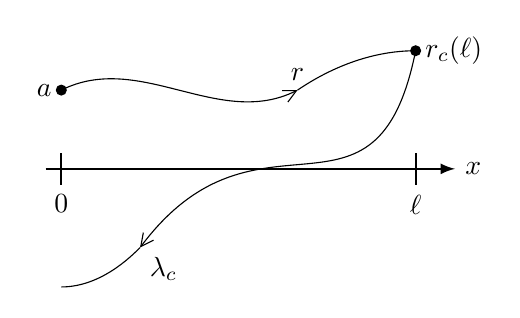
\begin{tikzpicture}
    \draw [thick,->] (-0.2,0) -- (5,0) node [anchor=west] {$x$};
    \draw [thick] (0,0.2) -- (0,-0.2) node [anchor=north] {$0$};
    \draw [thick] (4.5,0.2) -- (4.5,-0.2) node [anchor=north] {$\ell$};
    
    \node [dot] at (0,1) {};
    \node [dot] at (4.5,1.5) {};
    \draw [->,>={Straight Barb[scale length=2]}] (0,1) node [anchor=east] {$a$} .. controls (1,1.5) and (2,0.5) .. (3,1) node [anchor=south] {$r$};
    \draw (3,1) parabola [bend at end] (4.5,1.5) node [anchor=west] {$r_c(\ell)$};

    \draw [->,>={Straight Barb[scale length=2]}] (4.5,1.5) .. controls (4,-1) and (2.5,1) .. (1,-1) node [anchor=north west] {$\lambda_c$};
    \draw (1,-1) parabola [bend at end] (0,-1.5);
  \end{tikzpicture}
\end{center}
Problem: we can do this for any $c$. Which $c$ is it? \emph{Last 15 minutes was a dead end!}

Back to $u=F(r,\lambda)$. Assume we have $F$ (numerically).
\begin{align}
    \frac{\dif r}{\dif x} &= -F(r,\lambda) \\
    r(0) &= a \\
    \frac{\dif\lambda}{\dif x} &= -\frac{F^3(r,\lambda)}{1+F^2(r,\lambda)} \\
    \lambda(\ell) &= r(\ell)
\end{align}
The mistake before was that the simulation forward from $a$ depends on $\lambda$. 
\begin{center}
  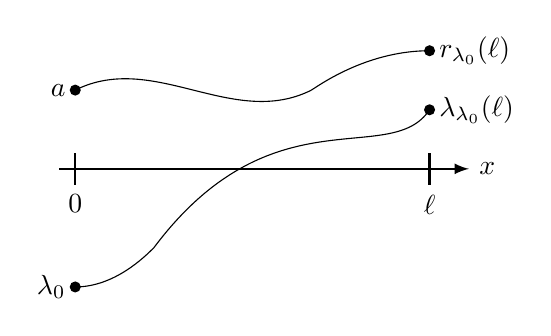
\begin{tikzpicture}
    \draw [thick,->] (-0.2,0) -- (5,0) node [anchor=west] {$x$};
    \draw [thick] (0,0.2) -- (0,-0.2) node [anchor=north] {$0$};
    \draw [thick] (4.5,0.2) -- (4.5,-0.2) node [anchor=north] {$\ell$};
    
    \node [dot] at (0,1) {};
    \node [dot] at (4.5,1.5) {};
    \draw [>={Straight Barb[scale length=2]}] (0,1) node [anchor=east] {$a$} .. controls (1,1.5) and (2,0.5) .. (3,1);
    \draw (3,1) parabola [bend at end] (4.5,1.5) node [anchor=west] {$r_{\lambda_0}(\ell)$};

    \node [dot] at (0,-1.5) {};
    \node [dot] at (4.5,0.75) {};
    \draw [>={Straight Barb[scale length=2]}] (4.5,0.75) node [anchor=west] {$\lambda_{\lambda_0}(\ell)$} .. controls (4,0) and (2.5,1) .. (1,-1);
    \draw (1,-1) parabola [bend at end] (0,-1.5) node [anchor=east] {$\lambda_0$};
  \end{tikzpicture}
\end{center}
Therefore, we should guess $\lambda_0$ and simulate both $r$ and $\lambda$ to get $r_{\lambda_0}(\ell)$ and $\lambda_{\lambda_0}(\ell)$. We need
\[ r_{\lambda_0}(\ell) = \lambda_{\lambda_0} \]
for optimality. To do this, we need numerics.

% 2017/02/09

\end{document}
